\documentclass[11pt]{article}
\usepackage[hmargin=1in,vmargin=1in]{geometry}
\usepackage{xcolor}
\usepackage{amsmath,amssymb,amsfonts,url,sectsty,framed,tcolorbox,framed} 
\usepackage[justification=centering]{caption}
\usepackage[labelformat=empty]{caption}
\usepackage{draftwatermark}
\usepackage{xcolor}
\usepackage{algorithm}
\usepackage{algpseudocode}
\usepackage{tikz}
\newcommand{\pf}{{\bf Proof: }}
\newtheorem{theorem}{Theorem}
\newtheorem{lemma}{Lemma}
\newtheorem{proposition}{Proposition}
\newtheorem{definition}{Definition}
\newtheorem{remark}{Remark}
\newcommand{\qed}{\hfill \rule{2mm}{2mm}}
\SetWatermarkText{\textcolor{gray!10}{202151188}}
\SetWatermarkScale{4}

\begin{document}
\setcounter{section}{0}
\noindent
\rule{\textwidth}{1pt}
\begin{center}
{\bf [CS304] Introduction to Cryptography and Network Security}
\end{center}
Course Instructor: Dr. Dibyendu Roy \hfill Winter 2023-2024\\
Scribed by: Dipean Dasgupta (202151188) \hfill Lecture 17,18 (Week 10)
\\
\rule{\textwidth}{1pt}

\section{Digital Signature Algorithms}
Digital signatures on documents and messages are created using Digital Signature Algorithms (DSA). A document will only be signed by you if you are using a DSA. All will be able to confirm your signature, nevertheless. The formal definition of a DSA is that it is a tuple (P, S, K, Sign, V) where, 
\begin{center}
    P $\rightarrow$ Plaintext \hspace{20pt}
    S $\rightarrow$ Signature Text \hspace{20pt}
    K $\rightarrow$ Key Space\\
    Sign $\rightarrow$ Signing Algorithm \hspace{20pt}
    V $\rightarrow$ Verification Algorithm\\
\end{center}
The signing algorithm Sign, takes plaintext P and a key from key space in order to generate a signature. i.e $Sign(p, k) = s$\\ 
The verification algorithm V takes p, s and k and produces output as 1 or 0 which can be written as:
\begin{center}
    (if s = sign(p,k))\\
    V(p, s, k) = 1 \\ 
    else 0 (othercases)
\end{center}
The RSA Signature technique is one such technique used for digital signatures.

\subsection{RSA Signature Algorithm}

\begin{align*}
& \textbf{Alice}\\
& PK: e, n \\
& SK: p, q, d \\
& S = m^d \ (\bmod\ n) 
\end{align*}
\hline
\begin{align*}
& \textbf{Bob}\\
& v = S^e \ (\bmod\ n) \\
& \text{if } v = m, \text{ output } 1 \\
& \text{else output } 0
\end{align*}


Bob and Alice would like to confirm Alice's digital signature after she signs a message. He would wish to sign the message $m$, and Alice will produce two huge primes, $p$ and $q$. Alice will calculate $n = p \cdot q \ and \phi(n) = (p-1) \cdot (q-1)$ using $p$ and $q$. To compute $d$, Alice will now select an integer $e$ such that $e \cdot d \equiv 1 \ mod \ \phi(n)$. Alice is going to sign the message in a way that makes it verifiable to others. Alice will compute,
\begin{center}
    Signing Algorithm: $S = m^d \ mod \ n$
\end{center}
Since $d$ is Alice's secret key, only Alice is able to do this calculation. Bob will receive $S$ from Alice. Using Alice's public key, $e$, which Bob knows, he will compute $v = S^e \mod \n$. The verification algorithm's output, 1, indicates that the signature has been validated if $v = m$. If not, it will produce 0. In order for Bob to be verified, he must be aware of the message $m$. You can transfer this message using any encryption scheme.\\
\newline
As you can see, with RSA, we computed $y = x^e \ mod \n$, or the recipient's public key, to encrypt the message, and we computed $x = y^d \ mod \n$, or the recipient's secret key, to decrypt it. However, the RSA Signature Algorithm uses the signee's (the person who must sign) secret key during signing and the signee's public key after verification. This indicates that the calculations for the RSA Signature Algorithm are different from those for RSA encryption and decryption. In each DSA, the signee's public key is used for verification while the signee's secret key is used for signing.\\
\newline

\subsection{RSA Encryption}
If two messages are encrypted using RSA, we get,
\begin{center}
    $c_1 = m_1^e \ mod \ n$\\
    $c_2 = m_2^e \ mod \ n$
\end{center}
If we multiply the two ciphertexts, we will get,
\begin{center}
    $c_1 \cdot c_2 = (m_1^e \cdot m_2^e) \ mod \ n = {(m_1 \cdot m_2)}^e \ mod \ n$
\end{center}
This makes it easy to see that the ciphertext for the message $m_1 \cdot m_2$ is $c_1 \cdot c_2$. Consequently, we can guarantee that the ciphertext for the message $m_1 \cdot m_2$ will be obtained by multiplying the two ciphertexts. Without actually encrypting the data, we can calculate the encryption of the multiplication of two messages. The term \textbf{Computation on Encrypted Data} refers to this mechanism.\\
\newline
It cannot be guaranteed that $c_1 + c_2$ will be the ciphertext for the message $m_1 + m_2$ if we only have $c_1$ and $c_2$. On the other hand, we can get the ciphertext of the message $a \cdot m$ without actually conducting the encryption if we multiply a constant $a$ to the message $m$ (matching ciphertext is c). The ciphertext for $a\cdot m$ will be $c$ multiplied by $a^e$.\\
\newline
There are certain algorithms for which additiom, multiplicaton and constant multiplication are possible. These are known as Fully Homomorphic Encryption Algorithms. RSA is not a fully homomorphic encryption algorithm as addition is not possible over RSA.\\
\newline
Similarly, if we consider two signatures,
\begin{center}
    $s_1 = m_1^d \ mod \ n$\\
    $s_2 = m_2^d \ mod \ n$
\end{center}
The signature on the message $m_1 \cdot m_2$ will be,
\begin{center}
    $s_1 \cdot s_2 = {(m_1 \cdot m_2)}^d \ mod \ n$
\end{center}
We shall receive a signature on the multiplication of two messages that can be independently verified by anybody. \textbf{Computation on the Authenticated Data} is the term for this.\\
\newline
Forging a signature on a message using the RSA Signature Algorithm is simple since it allows us to compute the signature on $m_1 \cdot m_2$ without actually signing. The message $m_1 \cdot m_2$ can be signed even if we don't truly know the signee's secret key.\\
\newline
To prevent the forging, the sign is done on the hash of the message.
\begin{center}
    $s_1 = {(h(m_1))}^d \ mod \ n$\\
    $s_2 = {(h(m_2))}^d \ mod \ n$
\end{center}
Now, if we try to multiply the two signatures, we will get,
\begin{center}
    $s_1 \cdot s_2 = {(h(m_1) \cdot h(m_2))}^d \ mod \ n$
\end{center}
Since, $h(m_1) \cdot h(m_2) \neq h(m_1 \cdot m_2)$, hence, 
\begin{center}
    $s_1 \cdot s_2 \neq {(h(m_1 \cdot m_2))}^d \ mod \ n$
\end{center}
Now, to verify, in verification algorithm, we compute,
\begin{center}
    $s_1^e \ mod \ n = h(m_1) \ mod \ n$
\end{center}
The message's verifier will be aware of $m_1$. After computing $h(m_1)$, the verifier will ascertain whether $s_1^e \ mod \ n = h(m_1) \ mod \ n$. Verification of the message occurs if they are equal. Only the signee's public key will be needed to validate the message.

\section{System of Modular Equations}
We will be solving a system of linear equations of the kind, where we have to find x, such that,
\begin{center}
    $a \cdot x \equiv b \ mod \ m$    (Eq.1)
\end{center}
 The above equation can be written as,
\begin{center}
    $a \cdot x - m \cdot y = b$     (Eq.2)
\end{center}
where y is an integer. From Bezout's Identiy we know that, 
\begin{center}
    $a \cdot x_0 + m \cdot y_0 = gcd(a, m)$    (Eq.3)
\end{center}
where $x_0$ and $y_0$ can be found using Extended Euclidean Algorithm.

If gcd(a, m) divides b, equation 2 can be solved; if not, there is no solution. Since b is divided by gcd(a, m), we can say,
\begin{center}
    $t \cdot gcd(a, m) = b$
\end{center}
Multiplying Eq.3 by t, we get, 
\begin{center}
    $a \cdot (t \cdot x_0) + m \cdot (t\cdot y_0) = t \cdot gcd(a, m) \implies a \cdot  X_0 + m \cdot Y_0 = b$
\end{center}

Thus, given an equation to solve, we shall first determine whether or not gcd(a, m) divides b. There is only a solution if it is splitting. Then, using the Extended Euclidean Algorithm, we will determine $x_0$ and $y_0$. We will then multiply these values by $t = \frac{b}{gcd(a, m)}$ to obtain $X_0$ and $Y_0$.\\
\newpage
If we know that $X_0$ and $Y_0$ are a solution of the Eq.2, then we can substitute x and y as, 
\begin{center}
    $x = X_0 + \frac{m}{gcd(a, m)} \cdot n$\\
    \vspace{1mm}
    $y = Y_0 + \frac{a}{gcd(a, m} \cdot n$
\end{center}
where n is an integer. The aforementioned x and y will satisfy Eq. 2 for any value of n. Thus, the generic solutions to Eq. 2 are x and y.\\
\newline
Now, let us consider a system of two modular equations,
\begin{center}
    $x \equiv a_1 \ mod \ m_1$   (Eq.1)\\
    $x \equiv a_2 \ mod \ m_2$   (Eq.2)  
\end{center}
where $m_1$ and $m_2$ are co-prime. It is required to find $x$ that satisfies both the equations. If $x$ is a solution of Eq.1, then.
\begin{center}
    $x = a_1 + m_1 \cdot y$  (Eq.3)
\end{center}
If $x$ is also a solution to Eq.2, then,
\begin{center}
    $x \equiv a_2 \ mod \ m_2$
\end{center}
Let us substitute the value of $x$ from Eq.3,
\begin{center}
    $a_1 + m_1 \cdot y \equiv a_2 \ mod \ m_2 \implies m_1 \cdot y \equiv (a_2 - a_1) \ mod \ m_2$   (Eq.4)
\end{center}
Since, gcd(m1, m2) = 1, therefore, from the general solution for only one equation above, we can say Eq.4 has the solution,
\begin{center}
    $y = y_0 + \frac{m_2}{gcd(m_1, m_2)} \cdot n \implies y = y_0 + m_2 \cdot n$
\end{center}
From Eq.3 we have, 
\begin{center}
    $x = a_1 + m_1 \cdot y \implies x = a_1 + m_1 \cdot (y_0 + m_2 \cdot n)$\\
    \vspace{1mm}
    $\implies x = (a_1 + m_1 \cdot y_0) + n \cdot m_1 \cdot m_2$
\end{center}
If we have $y_0$, let's say $x_0 = a_1 + m_1 \cdot y_0$, then,
\begin{center}
    $x = x_0 + m_1 \cdot m_2 \cdot n$\\
    \vspace{1mm}
    $x \equiv x_0 \ mod \ m_1 \cdot m_2$
\end{center}
Under $m_1 \cdot m_2$, $x_0$ is congruent modulo to any $x$. Every solution to the above system of equations will always be congruent to $x_0$ under modulo $m_1 \cdot m_2$ since $x$ is the universal solution of the two equations.
\newpage
\subsection{Chinese Remainder Theorem}
Consider the system of equations, 
\begin{center}
    $x \equiv a_1 \ mod \ m_1$\\
    $x \equiv a_2 \ mod \ m_2$\\
    .\\
    .\\
    $x \equiv a_r \ mod \ m_r$\\
\end{center}
where $m_1, m_2, \hdots, m_r$ are pairwise co-prime, then the above system has a unique solution modulo $(m_1 \cdot m_2 \hdots m_r)$. The proof for the above result is given below. For each $1 \leq j \leq r$, define $\delta_j$ as,
\begin{center}
    $\delta_j =$ 
     \begin{cases}
       \text{1,} &\quad\text{$mod \ m_j$}\\
       \text{0,} &\quad\text{$mod \ m_i, \ if\ i \neq j$}\\
     \end{cases}
\end{center}
Now, we can say that $x = \sum_{j=1}^r a_j \cdot \delta_j$ will satisfy the given system of equations. We are claiming that $x$ will satisfy all the equations. Let us expand $x$,
\begin{center}
    $x = \delta_1 \cdot a_1 + \delta_2 \cdot a_2 + \hdots + \delta_r \cdot a_r$ (Eq. 1)
\end{center}
Now, consider the $j^{th}$ equation in the given system of equations,
\begin{center}
    $x \equiv a_j \ mod \ m_j$
\end{center}
If we take modulus of $x$ under $m_j$, we will get,
\begin{center}
    $x \equiv (\delta_1 \cdot a_1 + \delta_2 \cdot a_2 + \hdots + \delta_r \cdot a_r) \ mod \ m_j$
\end{center}
All the $\delta_i, \ for \ i \neq j$ will be 0, and also, $\delta_j = 1$, from the definition of $\delta$. Therefore, 
\begin{center}
    $x \equiv a_j \ mod \ m_j$
\end{center}
Given that we know $\delta_j$, we can therefore conclude that $x$ is a solution to the system of equations. Now, let us find $\delta_j \ for \ 1 \leq j \leq r$. Let us say the integer M is equal to:
\begin{center}
    $M = m_1 \cdot m_2 \hdots m_r$
\end{center}
Our goal is to compute the $gcd(\frac{M}{m_j}, m_j)$. It will obviously equal 1 as $m_i$ are pairwise co-prime. Since $M$ is the product of all $m_i$, $\frac{M}{m_j}$ does not include $m_j$. Hence,
\begin{center}
    $gcd(\frac{M}{m_j}, m_j) = 1$
\end{center}
This indicates that $\frac{M}{m_j}$ has an inverse that we can find under modulo $m_j$. Let $b_j$ be $\frac{M}{m_j}$'s multiplicative inverse, modulo $m_j$. Then, 
\begin{center}
    $\frac{M}{m_j} \cdot b_j \equiv 1 \ mod \ m_j$
\end{center}
We can use the Extended Euclidean Algorithm to find $b_j$. Now, $delta_j$ is defined as:
\begin{center}
    $\delta_j = \frac{M}{m_j} \cdot b_j$
\end{center}
It is obvious that the residual after dividing $\delta_j$ by $m_j$ will be 1. Moreover, the remainder will be 0 if we divide $\delta_j$ by any $m_i, i \neq j$. We can check it as follows.
\begin{center}
    $\delta_j \ mod \ m_i = \frac{M}{m_j} \cdot b_j \ (mod \ m_i)$\\
    \vspace{1mm}
    $\delta_j \ mod \ m_i = \{\frac{m_1 \cdot m_2 \hdots m_{j-1} \cdot m_{j+1} \hdots m_i \cdot m_{i+1} \hdots m_r}{m_j} \cdot b_j\} \ mod \ m_i$\\
    \vspace{1mm}
    $\delta_j \ mod \ m_i = t \cdot m_i \ (mod \ m_i) = 0$
\end{center}
Therefor, the solution is $x = \sum_{j=1}^r a_j \cdot \delta_j$, where $\delta_j$ is,
\begin{center}
    $\delta_j =$ 
     \begin{cases}
       \text{1,} &\quad\text{$mod \ m_j$}\\
       \text{0,} &\quad\text{$mod \ m_i, \ if\ i \neq j$}\\
     \end{cases}
\end{center}

To solve a given system of equations, follow the steps:
\begin{enumerate}
    \item Check if $m_i$ are pairwise co-prime. If yes, continue to next step.
    \item Calculate $M = m_1 \cdot m_2 \hdots m_r$
    \item Calculate $b_j$ for each $\frac{M}{m_j}$ under modulo $m_j$.
    \item Calculate $\delta_j = \frac{M}{m_j} \cdot b_j$
    \item Calculate $x = \sum_{j=1}^r a_j \cdot \delta_j$
    \item Optionally, you can verify your solution by putting the value of $x$ in each equation.
\end{enumerate}
\textbf{Uniqueness of Solution}\\
We shall now demonstrate the solution's uniqueness. Assuming $x'$ to be an additional solution to the provided system of equations, we can infer from our conclusion regarding a system of two equations that all solutions will be congruent to $x_0$ if we know a solution for $x_0$. Therefore, 
\begin{center}
    $x' \equiv x \ mod \ (m_1 \cdot m_2 \hdots m_r)$
\end{center}
Since, $x \ and \ x'$ are solutions of the system of equations then for any equation we can say,
\begin{center}
    $x \equiv a_i \ mod \ m_i$\\
    $x' \equiv a_i \ mod \ m_i$
\end{center}
If we subtract the above two equations, we will get,
\begin{center}
    $x' - x \equiv 0 \ mod \ m_i \implies x' \equiv x \ mod \ m_i, 1 \leq i \leq r$
\end{center}
Since, $(x' - x)$ is divisible by each $m_i$ and $m_i$ are pairwise co-prime, we can conclude that,
\begin{center}
    $x' \equiv x \ mod \ (m_1 \cdot m_2 \hdots m_r)$
\end{center}
Hence, the solution is unique under modulo $(m_1 \cdot m_2 \hdots m_r)$.

\section{Elliptic Curve Cryptography}
We only need to employ the Square and Multiply Algorithms; RSA was really simple in that way. The Square and Multiply Algorithm makes computations incredibly simple, and the rigorous procedures that ensure accuracy and security are similarly simple.\\
\newline
We're going to define elliptic curve cryptography right now. Instead of using integers for the calculations in this case, we will use a curve. From there, we can see that we can create the currently in use Diffie-Hellman Key Exchange and Signature algorithms. Elliptic Curve Diffie-Hellman (ECDH) is used for the key exchange, and Elliptic Curve Digital Signature Algorithm (ECDSA) is used for signatures. We utilize Elliptic Curve techniques rather than RSA because they offer more security while requiring a comparatively smaller prime value.\\
\newline
Let's examine the operation of elliptic curve cryptography. Since cryptography is always built on discrete systems, we will start with real numbers and create a discrete structure from there.\\
\newline
Let's define two number a and b such that,
\begin{center}
    $a, b \in \mathbb{R} \ and \ 4a^3 + 27b^2 \neq 0$
\end{center}
Let us define a curve,
\begin{center}
    $y^2 = x^3 + ax + b$
\end{center}
where $(x,y) \in \mathbb{R}_2$. This curve is called as the Elliptic Curve. If we draw the curve, there will be two structures, one is shown below, and the other will be discussed later.
\begin{center}
    \tikzset{every picture/.style={line width=0.75pt}}
    \begin{tikzpicture}[x=0.75pt,y=0.75pt,yscale=-1,xscale=1]
        \draw    (105,213) -- (498,213) ;
        \draw [shift={(500,213)}, rotate = 180] [color={rgb, 255:red, 0; green, 0; blue, 0 }  ][line width=0.75]    (10.93,-3.29) .. controls (6.95,-1.4) and (3.31,-0.3) .. (0,0) .. controls (3.31,0.3) and (6.95,1.4) .. (10.93,3.29)   ;
        \draw [shift={(103,213)}, rotate = 0] [color={rgb, 255:red, 0; green, 0; blue, 0 }  ][line width=0.75]    (10.93,-3.29) .. controls (6.95,-1.4) and (3.31,-0.3) .. (0,0) .. controls (3.31,0.3) and (6.95,1.4) .. (10.93,3.29)   ;
 
        \draw    (292.01,49) -- (292.99,373) ;
        \draw [shift={(293,375)}, rotate = 269.83] [color={rgb, 255:red, 0; green, 0; blue, 0 }  ][line width=0.75]    (10.93,-3.29) .. controls (6.95,-1.4) and (3.31,-0.3) .. (0,0) .. controls (3.31,0.3) and (6.95,1.4) .. (10.93,3.29)   ;
        \draw [shift={(292,47)}, rotate = 89.83] [color={rgb, 255:red, 0; green, 0; blue, 0 }  ][line width=0.75]    (10.93,-3.29) .. controls (6.95,-1.4) and (3.31,-0.3) .. (0,0) .. controls (3.31,0.3) and (6.95,1.4) .. (10.93,3.29)   ;
 
        \draw    (373,320) .. controls (375.42,318.19) and (373,309) .. (371.45,307.24) .. controls (369.91,305.47) and (182,291) .. (182,213) .. controls (182,135) and (364,117) .. (364.24,103.33) .. controls (364.49,89.66) and (360.53,97.04) .. (365,96) ;

        \draw (506,201) node [anchor=north west][inner sep=0.75pt]   [align=left] {x};
        \draw (295,31) node [anchor=north west][inner sep=0.75pt]   [align=left] {y};
        \draw (163,189) node [anchor=north west][inner sep=0.75pt]   [align=left] {A};
    \end{tikzpicture}
\end{center}
At point A, $y = 0 \impies x^3 + ax + b = 0$ (Eq.1). This equation will have three roots and the roots will be either:
\begin{itemize}
    \item three real roots
    \item one real root, two complex roots
\end{itemize}
Eq.1 will have three distinct root iff $4a^3 + 27b^2 \neq 0$ (can be real or complex). If we consider the above curve and put y = 0, we can see that it will have only one real root and two complex roots.\\
\newpage

Let us define some properties on the curve we defined before.
\begin{center}
    \tikzset{every picture/.style={line width=0.75pt}} 
    \begin{tikzpicture}[x=0.75pt,y=0.75pt,yscale=-1,xscale=1]
        \draw    (105,213) -- (498,213) ;
        \draw [shift={(500,213)}, rotate = 180] [color={rgb, 255:red, 0; green, 0; blue, 0 }  ][line width=0.75]    (10.93,-3.29) .. controls (6.95,-1.4) and (3.31,-0.3) .. (0,0) .. controls (3.31,0.3) and (6.95,1.4) .. (10.93,3.29)   ;
        \draw [shift={(103,213)}, rotate = 0] [color={rgb, 255:red, 0; green, 0; blue, 0 }  ][line width=0.75]    (10.93,-3.29) .. controls (6.95,-1.4) and (3.31,-0.3) .. (0,0) .. controls (3.31,0.3) and (6.95,1.4) .. (10.93,3.29)   ; 
        \draw    (292.01,49) -- (292.99,373) ;
        \draw [shift={(293,375)}, rotate = 269.83] [color={rgb, 255:red, 0; green, 0; blue, 0 }  ][line width=0.75]    (10.93,-3.29) .. controls (6.95,-1.4) and (3.31,-0.3) .. (0,0) .. controls (3.31,0.3) and (6.95,1.4) .. (10.93,3.29)   ;
        \draw [shift={(292,47)}, rotate = 89.83] [color={rgb, 255:red, 0; green, 0; blue, 0 }  ][line width=0.75]    (10.93,-3.29) .. controls (6.95,-1.4) and (3.31,-0.3) .. (0,0) .. controls (3.31,0.3) and (6.95,1.4) .. (10.93,3.29)   ; 
        \draw    (362,317.4) .. controls (355,310.4) and (360,309.4) .. (347,304.4) .. controls (334,299.4) and (182,291) .. (182,213) .. controls (182,135) and (359.76,119.07) .. (360,105.4) .. controls (360.24,91.73) and (368,91.4) .. (362,94.4) ; 
        \draw [color={rgb, 255:red, 245; green, 166; blue, 35 }  ,draw opacity=1 ]   (217,160) -- (218,267.4) ; 
        \draw [color={rgb, 255:red, 208; green, 2; blue, 27 }  ,draw opacity=1 ]   (362,94.4) -- (217,160) ; 
        \draw [color={rgb, 255:red, 65; green, 117; blue, 5 }  ,draw opacity=1 ]   (275,132.4) -- (275,289.4) ;
        \draw [color={rgb, 255:red, 189; green, 16; blue, 224 }  ,draw opacity=1 ]   (362,94.4) -- (362,317.4) ;
        
        \draw (506,201) node [anchor=north west][inner sep=0.75pt]   [align=left] {x};
        \draw (295,31) node [anchor=north west][inner sep=0.75pt]   [align=left] {y};
        \draw (160,132) node [anchor=north west][inner sep=0.75pt]   [align=left] {$P (x_1, y_1)$};
        \draw (226,103) node [anchor=north west][inner sep=0.75pt]   [align=left] {$Q (x_2, y_2)$};
        \draw (142,269) node [anchor=north west][inner sep=0.75pt]   [align=left] {$-P (x_1, -y_1)$};
        \draw (214,298) node [anchor=north west][inner sep=0.75pt]   [align=left] {$-Q (x_2, -y_2)$};
        \draw (368,79) node [anchor=north west][inner sep=0.75pt]   [align=left] {-R};
        \draw (377,317) node [anchor=north west][inner sep=0.75pt]   [align=left] {R};
    \end{tikzpicture}
\end{center}
If we unite two points P and Q on the curve with a straight line, we will cut the curve again at a point, say -R. The point -X is the mirror image of X, using the x-axis as a mirror. Alternatively, we might state that the perpendicular from point X to the x-axis will cut the curve again at point -X.
\begin{enumerate}
    \item $P \  \boxed{+}  \ Q = R$. The binary operator $\boxed{+}$ is described as taking two points and joining them using a straight line. The line will intersect the curve again at some time. The output point is represented by its picture on the x-axis.
    \item $\Theta$ is referred to as the point of infinity. If we combine P and -P, the resulting straight line will be parallel to the y-axis. The elliptic curve is infinite, and we assume that the straight line will intersect the curve at one point, which will be the point of infinity.
    \item $P \ \boxed{+} -P = \Theta$
    \item ${P \ \boxed{+} \ \Theta = P}$
    \item $(P \ \boxed{+} \ Q) \ \boxed{+} \ R = P \ \boxed{+} \ (Q \ \boxed{+} \ R)$
    \item $P \ \boxed{+} \ Q = Q \ \boxed{+} \ P$
    
\end{enumerate}
Using a graphical tool, one may demonstrate the associativity and commutativity of the $\boxed{+}$ operator. Consider $\Theta$ as the identity element and $-P$ as its inverse. Hence, the curve with the $\boxed{+}$ operator forms a commutative group.\\
\newline
If we need to find $P \ \boxed{+} P$, we draw the tangent to the curve at P, and wherever the tangent cuts the curve again, the picture on the x-axis represents the result. $P \ \boxed{+} = R \implies 2P = R$. Let us see it in the graph:
\begin{center}
\tikzset{every picture/.style={line width=0.75pt}}       
    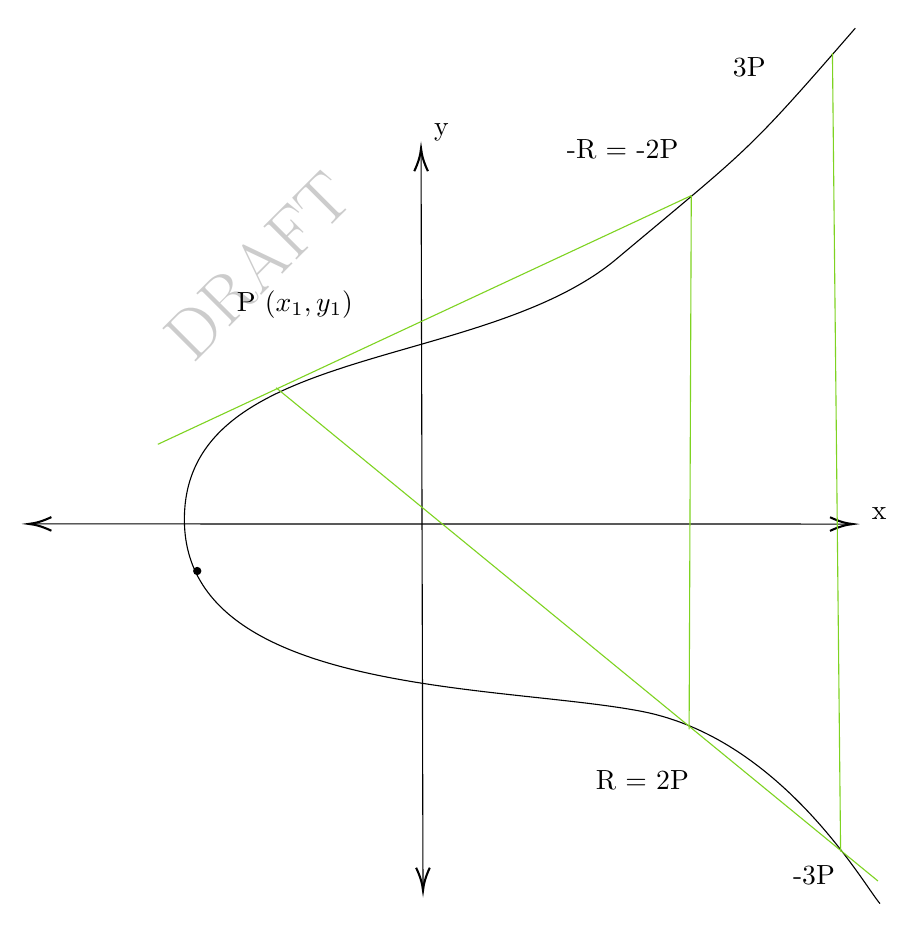
\begin{tikzpicture}[x=0.75pt,y=0.75pt,yscale=-1,xscale=1]
        \draw    (105,268.22) -- (498,268.29) ;
        \draw [shift={(500,268.29)}, rotate = 180.01] [color={rgb, 255:red, 0; green, 0; blue, 0 }  ][line width=0.75]    (10.93,-3.29) .. controls (6.95,-1.4) and (3.31,-0.3) .. (0,0) .. controls (3.31,0.3) and (6.95,1.4) .. (10.93,3.29)   ;
        \draw [shift={(103,268.22)}, rotate = 0.01] [color={rgb, 255:red, 0; green, 0; blue, 0 }  ][line width=0.75]    (10.93,-3.29) .. controls (6.95,-1.4) and (3.31,-0.3) .. (0,0) .. controls (3.31,0.3) and (6.95,1.4) .. (10.93,3.29)   ;
        \draw    (292.03,89.34) -- (292.96,442.8) ;
        \draw [shift={(292.97,444.8)}, rotate = 269.85] [color={rgb, 255:red, 0; green, 0; blue, 0 }  ][line width=0.75]    (10.93,-3.29) .. controls (6.95,-1.4) and (3.31,-0.3) .. (0,0) .. controls (3.31,0.3) and (6.95,1.4) .. (10.93,3.29)   ;
        \draw [shift={(292.02,87.34)}, rotate = 89.85] [color={rgb, 255:red, 0; green, 0; blue, 0 }  ][line width=0.75]    (10.93,-3.29) .. controls (6.95,-1.4) and (3.31,-0.3) .. (0,0) .. controls (3.31,0.3) and (6.95,1.4) .. (10.93,3.29)   ;
        \draw    (513.17,451.17) .. controls (506.17,443.54) and (466.18,371.6) .. (398.18,358.51) .. controls (330.18,345.42) and (177.98,351.06) .. (178,266.05) .. controls (178.01,181.04) and (321.21,195.02) .. (386.22,140.54) .. controls (451.22,86.06) and (448.22,90.42) .. (501.23,29.4) ;
        \draw [color={rgb, 255:red, 126; green, 211; blue, 33 }  ,draw opacity=1 ]   (165.2,229.87) -- (422.22,110.03) ;
        \draw [color={rgb, 255:red, 126; green, 211; blue, 33 }  ,draw opacity=1 ]   (422.22,110.03) -- (421.18,367.23) ; 
        \draw  [line width=3] [line join = round][line cap = round] (184.19,290.9) .. controls (184.19,290.9) and (184.19,290.9) .. (184.19,290.9) ; 
        \draw [color={rgb, 255:red, 126; green, 211; blue, 33 }  ,draw opacity=1 ]   (222.21,202.63) -- (512.17,440.27) ;
        \draw [color={rgb, 255:red, 126; green, 211; blue, 33 }  ,draw opacity=1 ]   (490.23,41.39) -- (494.17,426.1) ;
        
        \draw (508,259.25) node [anchor=north west][inner sep=0.75pt]  [rotate=-0.01] [align=left] {x};
        \draw (297.03,73.94) node [anchor=north west][inner sep=0.75pt]  [rotate=-0.01] [align=left] {y};
        \draw (202.01,154.57) node [anchor=north west][inner sep=0.75pt]  [rotate=-0.01] [align=left] {P $(x_1, y_1)$};
        \draw (361.03,81.58) node [anchor=north west][inner sep=0.75pt]  [rotate=-0.01] [align=left] {\mbox{-}R = -2P};
        \draw (374.98,385.64) node [anchor=north west][inner sep=0.75pt]  [rotate=-0.01] [align=left] {R = 2P};
        \draw (469.97,431.43) node [anchor=north west][inner sep=0.75pt]  [rotate=-0.01] [align=left] {\mbox{-}3P};
        \draw (441.03,42.36) node [anchor=north west][inner sep=0.75pt]  [rotate=-0.01] [align=left] {3P};
        
    \end{tikzpicture}
\end{center}

In the figure above, P and P coincide, and we draw the tangent to obtain its image. To find 3P, we can use the equation $2P \ \boxed{+} P$, as shown in the picture. So, NP = $(N-1)P \ \boxed{+} P$. \\
\subsubsection{Mathematical Aspects}
\underline{Elliptic Curve:}\\
\begin{center}
    $y^2\ =\ x^3+ax+b$\\
    \vspace{1mm}
    $4a^3+27b^2\ \neq 0$
\end{center}
Let us consider two points P($x_1, y_1$) and Q($x_2, y_2$). We have three cases,
\begin{enumerate}
    \item $x_1\neq x_2$, $y_1\neq y_2$
    \item $x_1= x_2$, $y_1=\  -y_2$
    \item $x_1= x_2$, $y_1= y_2$
    
\end{enumerate}
\begin{center}
    \tikzset{every picture/.style={line width=0.75pt}}       

    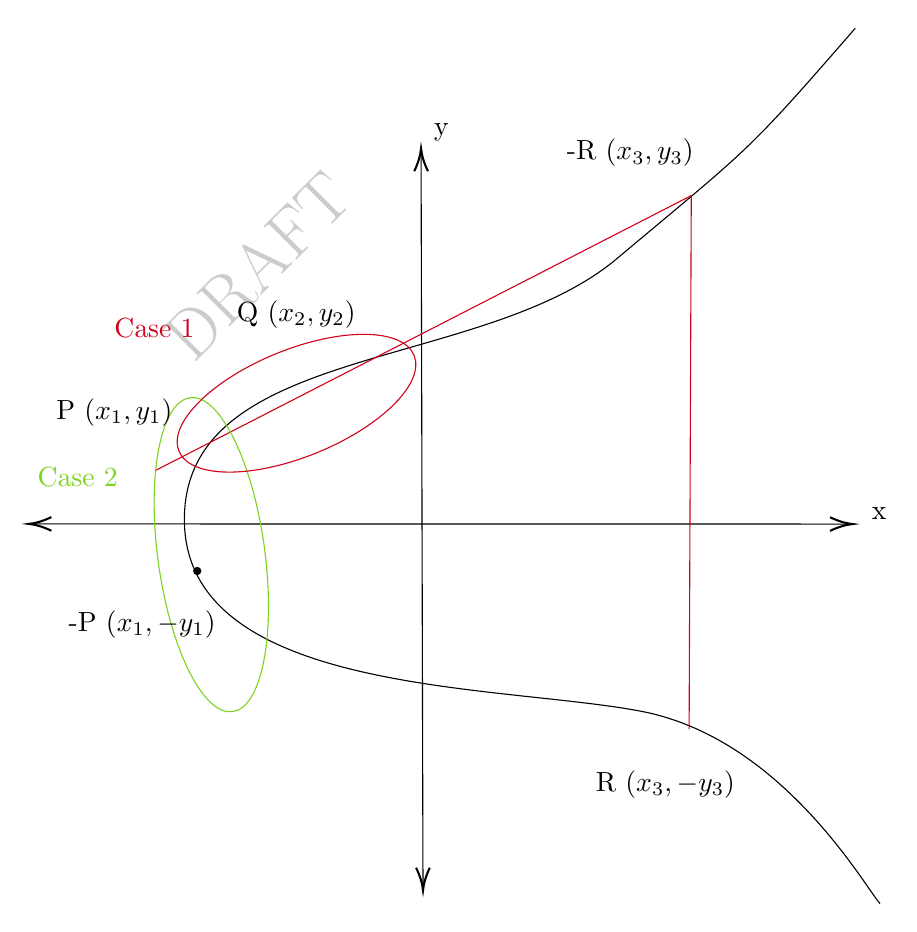
\begin{tikzpicture}[x=0.75pt,y=0.75pt,yscale=-1,xscale=1]
    \draw    (105,268.22) -- (498,268.29) ;
    \draw [shift={(500,268.29)}, rotate = 180.01] [color={rgb, 255:red, 0; green, 0; blue, 0 }  ][line width=0.75]    (10.93,-3.29) .. controls (6.95,-1.4) and (3.31,-0.3) .. (0,0) .. controls (3.31,0.3) and (6.95,1.4) .. (10.93,3.29)   ;
    \draw [shift={(103,268.22)}, rotate = 0.01] [color={rgb, 255:red, 0; green, 0; blue, 0 }  ][line width=0.75]    (10.93,-3.29) .. controls (6.95,-1.4) and (3.31,-0.3) .. (0,0) .. controls (3.31,0.3) and (6.95,1.4) .. (10.93,3.29)   ;
    \draw    (292.03,89.34) -- (292.96,442.8) ;
    \draw [shift={(292.97,444.8)}, rotate = 269.85] [color={rgb, 255:red, 0; green, 0; blue, 0 }  ][line width=0.75]    (10.93,-3.29) .. controls (6.95,-1.4) and (3.31,-0.3) .. (0,0) .. controls (3.31,0.3) and (6.95,1.4) .. (10.93,3.29)   ;
    \draw [shift={(292.02,87.34)}, rotate = 89.85] [color={rgb, 255:red, 0; green, 0; blue, 0 }  ][line width=0.75]    (10.93,-3.29) .. controls (6.95,-1.4) and (3.31,-0.3) .. (0,0) .. controls (3.31,0.3) and (6.95,1.4) .. (10.93,3.29)   ; 
    \draw    (513.17,451.17) .. controls (506.17,443.54) and (466.18,371.6) .. (398.18,358.51) .. controls (330.18,345.42) and (177.98,351.06) .. (178,266.05) .. controls (178.01,181.04) and (321.21,195.02) .. (386.22,140.54) .. controls (451.22,86.06) and (448.22,90.42) .. (501.23,29.4) ;
    \draw [color={rgb, 255:red, 208; green, 2; blue, 27 }  ,draw opacity=1 ]   (164.2,242.4) -- (422.22,110.03) ;
    \draw [color={rgb, 255:red, 208; green, 2; blue, 27 }  ,draw opacity=1 ]   (422.22,110.03) -- (421.18,367.23) ;
    \draw  [line width=3] [line join = round][line cap = round] (184.19,290.9) .. controls (184.19,290.9) and (184.19,290.9) .. (184.19,290.9) ;
    \draw  [color={rgb, 255:red, 126; green, 211; blue, 33 }  ,draw opacity=1 ] (201.23,358.68) .. controls (187.11,360.59) and (171.08,328.28) .. (165.42,286.51) .. controls (159.75,244.74) and (166.61,209.33) .. (180.73,207.41) .. controls (194.84,205.5) and (210.88,237.81) .. (216.54,279.58) .. controls (222.2,321.35) and (215.35,356.77) .. (201.23,358.68) -- cycle ;
    \draw  [color={rgb, 255:red, 208; green, 2; blue, 27 }  ,draw opacity=1 ] (175.36,233.11) .. controls (169.99,219.91) and (191.01,198.9) .. (222.3,186.17) .. controls (253.59,173.45) and (283.31,173.83) .. (288.67,187.03) .. controls (294.04,200.22) and (273.02,221.24) .. (241.73,233.96) .. controls (210.44,246.69) and (180.72,246.31) .. (175.36,233.11) -- cycle ;

    \draw (508,259.25) node [anchor=north west][inner sep=0.75pt]  [rotate=-0.01] [align=left] {x};
    \draw (297.03,73.94) node [anchor=north west][inner sep=0.75pt]  [rotate=-0.01] [align=left] {y};
    \draw (115.01,206.57) node [anchor=north west][inner sep=0.75pt]  [rotate=-0.01] [align=left] {P ($x_1, y_1$)};
    \draw (361.03,81.58) node [anchor=north west][inner sep=0.75pt]  [rotate=-0.01] [align=left] {\mbox{-}R ($x_3, y_3$)};
    \draw (374.98,385.64) node [anchor=north west][inner sep=0.75pt]  [rotate=-0.01] [align=left] {R ($x_3, -y_3$)};
    \draw (202.01,159.57) node [anchor=north west][inner sep=0.75pt]  [rotate=-0.01] [align=left] {Q ($x_2, y_2$)};
    \draw (121.01,308.57) node [anchor=north west][inner sep=0.75pt]  [rotate=-0.01] [align=left] {\mbox{-}P ($x_1, -y_1$)};
    \draw (143,168) node [anchor=north west][inner sep=0.75pt]   [align=left] {\textcolor[rgb]{0.82,0.01,0.11}{Case 1}};
    \draw (106,240) node [anchor=north west][inner sep=0.75pt]   [align=left] {\textcolor[rgb]{0.49,0.83,0.13}{Case 2}};
    \end{tikzpicture}
\end{center}

\textbf{\underline{Case-1:}}\\
\begin{center}
    y = mx + c              ...Eqn(a)\\
    \vspace{1mm}
    m = $\frac{y_2-y_1}{x_2-x_1}$\\
    \vspace{1mm}
    $y_1$ = $mx_1$ + c\\
    \vspace{1mm}
    $\implies$ $c = y_1-mx_1$, $c = y_2-mx_2$\\
\end{center}
All the points on this line will satisfy this equation of straight line. Equation of straight line(Eqn(a)) will cut the curve at a point, so we substitute value of y in the curve equation.
\begin{center}
    $y_2=x_3+ax+b$\\
    \vspace{1mm}
    ${(mx+c)}^2 = x_3+ax+b$\\
    \vspace{1mm}
    $m^2x^2+2mxc+c^2 = x_3+ax+b$\\
    \vspace{1mm}
    $x^3-m^2x^2+(a-2mc)x+(b-c^2)=0$\\
\end{center}
We already know that $(x_1,y_1),(x_2,y_2)$ will satisfy this equation. If $x_3$ is another solution of the above system, then,
\begin{center}
    $x_1+x_2+x_3=m^2$\\
    \vspace{1mm}
    $\implies$ $x_3=m^2-x_1-x_2$\\
    \vspace{3mm}
    We already know that m = $\frac{y_2-y_1}{x_2-x_1}$ = $\frac{y_3-y_1}{x_3-x_1}$\\
    \vspace{3mm}
    $\implies$ $y_3=y_1+m(x_3-x_1)$\\
\end{center}
So, we see that we obtained co-ordinate of R($x_3,y_3)$
\begin{center}
    $P \ \boxed{+} Q\ =\ R$
\end{center}
\textbf{\underline{Case-2:}}
\begin{center}
    P = $(x_1,y_1)$\\
    \vspace{1mm}
    Q = $(x_2,y_2)$\\
    \vspace{1mm}
    where $x_1=x_2, y_1=-y_2$\\
    \vspace{1mm}
    In this case $P \ \boxed{+} Q\ =\ \theta$\\
\end{center}

\textbf{\underline{Case-3:}}
\begin{center}
    P = $(x_1,y_1)$\\
    Q = $(x_2,y_2)$\\
    where $x_1=x_2, y_1=y_2$\\
\end{center}

\begin{center}
    $y = mx+c$\\
    \vspace{1mm}
    $y_2=x_3+ax+b$\\
    \vspace{1mm}
    $\implies$ $2y\frac{dy}{dx}\ =\ 3x^2+a$\\
    \vspace{1mm}
    $\implies$ $\frac{dy}{dx}\ =\ \frac{3x^2+a}{2y}$\\
    \vspace{1mm}
    ${(\frac{dy}{dx})}_{(x_1,y_1)}$ = $\frac{3{x_1}^2+a}{2y_1}$ = m\\
    \vspace{3mm}
    c = $y_1-mx_1$\\
\end{center}
Let us substitute in curve
\begin{center}
    $y_2=x_3+ax+b$\\
    $\implies$${(mx+c)}^2 = x_3+ax+b$\\
    $x_1+x_2+x_3=m^2$\\
    $\implies$$x_3=m^2-x_1-x_2$\\
    $m = \frac{y_3-y_1}{x_3-x_1}$\\
    $\implies$ $y_3 = y_1+m(x_3-x_1)$\\
    R$\rightarrow(x_3,-y_3)$\\
\end{center}
Now, let us consider the same curve in $\mathbb{Z_P}\ \times\ \mathbb{Z_P}$, where P is a prime number.
\begin{center}
    $y^2=x^3+ax+b$, where (x,y)$\in$ $\mathbb{Z_P}\ \times\ \mathbb{Z_P}$ and a, b $\in\ \mathbb{Z_P}$\\
    \vspace{1mm}
    $4a^3+27b^2\ \neq\ 0\ mod\ P$\\
\end{center}
As we are now working on discrete values, we will not obtain a curve, instead we will obtain points.\\
\textbf{\underline{Case-1:}}\\
\begin{center}
    $x^3=m^2-x_1-x_2$\\
    \vspace{1mm}
    $m = \frac{y_2-y_1}{x_2-x_1}$\\
\end{center}
We do not divide here; instead, we take the inverse modulo P. Because $x_2, x_1$ are distinct values, $x_2-x_1$ will be non-zero, and we will be able to determine its inverse under mod P because P is prime, therefore its gcd with ($x_2-x_1)$ will be 1.
\begin{center}
     $m = (y_2-y_1)\times{(x_2-x_1)}^{-1}\ mod P$\\
     \vspace{1mm}
     $\implies$ $y_3=y_1+m(x_3-x_1)\ \in\ \mathbb{Z_P}$\\
\end{center}

\subsubsection{Elliptic Curve Diffie-Hellman(ECDH)}
Let us now consider a scenario, where Alice and Bob want to exchange the messages. They have a curve E and a point P and (E, P) is public.
\begin{center}        
    \tikzset{every picture/.style={line width=0.75pt}}       
    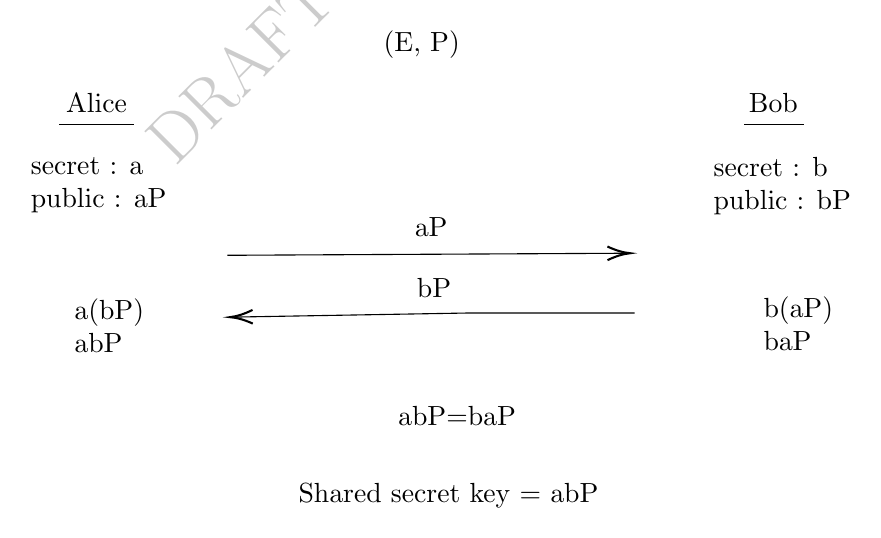
\begin{tikzpicture}[x=0.75pt,y=0.75pt,yscale=-1,xscale=1]
        \draw    (137,64.4) -- (173,64.4) ;
        \draw    (467,64.4) -- (496,64.4) ; 
        \draw    (218,127.4) -- (319.21,126.88) -- (410,126.41) ;
        \draw [shift={(412,126.4)}, rotate = 179.7] [color={rgb, 255:red, 0; green, 0; blue, 0 }  ][line width=0.75]    (10.93,-3.29) .. controls (6.95,-1.4) and (3.31,-0.3) .. (0,0) .. controls (3.31,0.3) and (6.95,1.4) .. (10.93,3.29)   ; 
        \draw    (414.2,155.2) -- (334.2,155.2) -- (221.2,157.17) ;
        \draw [shift={(219.2,157.2)}, rotate = 359] [color={rgb, 255:red, 0; green, 0; blue, 0 }  ][line width=0.75]    (10.93,-3.29) .. controls (6.95,-1.4) and (3.31,-0.3) .. (0,0) .. controls (3.31,0.3) and (6.95,1.4) .. (10.93,3.29)   ;
    
        \draw (139,48) node [anchor=north west][inner sep=0.75pt]   [align=left] {Alice};
        \draw (468,48) node [anchor=north west][inner sep=0.75pt]   [align=left] {Bob};
        \draw (122,79) node [anchor=north west][inner sep=0.75pt]   [align=left] {secret : a\\public : aP};
        \draw (292,18) node [anchor=north west][inner sep=0.75pt]   [align=left] {(E, P)};
        \draw (451,79) node [anchor=north west][inner sep=0.75pt]   [align=left] {secret : b\\public : bP};
        \draw (307,108) node [anchor=north west][inner sep=0.75pt]   [align=left] {aP};
        \draw (308,137) node [anchor=north west][inner sep=0.75pt]   [align=left] {bP};
        \draw (143,147) node [anchor=north west][inner sep=0.75pt]   [align=left] {a(bP)\\abP};
        \draw (475,146) node [anchor=north west][inner sep=0.75pt]   [align=left] {b(aP)\\baP};
        \draw (299,199) node [anchor=north west][inner sep=0.75pt]   [align=left] {abP=baP};
        \draw (251,236) node [anchor=north west][inner sep=0.75pt]   [align=left] {Shared secret key = abP};
        
    \end{tikzpicture}
\end{center}
In the preceding case, E and P were public, although a and b were secret. Because a, b, and P are all discrete, we may calculate aP (a times P), bP (b times P), and so on. Because they are discrete, abP and baP are identical. Alice and Bob have successfully exchanged messages now that they have reached the same place on the curve.\\
\newline
\textbf{Note:} Security of ECDH depends on the fact that finding xP from P is computationally difficult. This hard problem is known as \textbf{Discrete log problem on EC}.
\underline{Note:} We can plot and see the elliptic curve calculations on Jupyter Notebook. We can get the codes from the website called Sagehelp.
\subsubsection{Elliptic Curve Digital Signature Algorithm(ECDSA)}
Let us first recall the RSA and RSA Signature Algorithm,
\begin{center}
    \begin{itemize}
        \item RSA Encryption/Decryption:\\
        Encryption : c = $x^e$ mod n\\
        Decryption : x = $c^d$ mod n\\
    
        \item RSA Signature Algorithm:\\
        Signature : s = $x^d$ mod n\\
        Verification : x = $s^e$ mod n\\
    \end{itemize}
\end{center}

In ECDSA, we have (E, P) as public keys.\\
    Secret Key : a\\
    Public Key : aP\\
Here, we need 
\begin{itemize}
    \item elliptic curve EC
    \item a base point-G on the curve. G is such that there exists a large prime number n, such that
\end{itemize}
\begin{center}
    $n\cdotG = 0$\\
    $\implies$ $(n-1)G\ \boxed{+} G\ =\ nG$\\
\end{center}
\begin{center}
    Secret Key : $d_A$\\
    Public Key $Q_A$ : $d_A$
\end{center}
Now let us see a scenario between Alice and Bob:
\begin{center}
    \tikzset{every picture/.style={line width=0.75pt}}         
    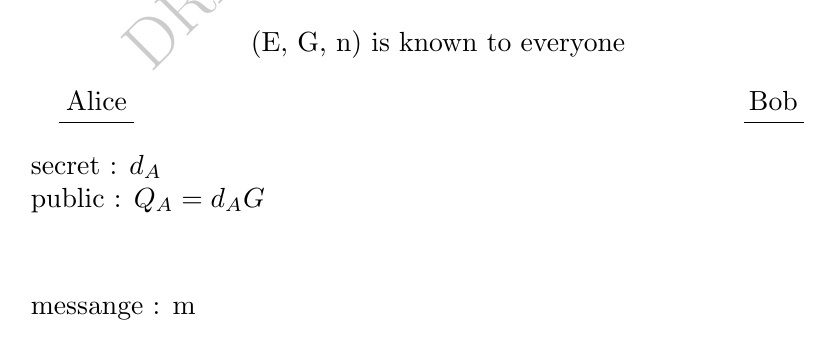
\begin{tikzpicture}[x=0.75pt,y=0.75pt,yscale=-1,xscale=1]
        \draw    (137,64.4) -- (173,64.4) ;
        \draw    (467,64.4) -- (496,64.4) ;
        
        \draw (139,48) node [anchor=north west][inner sep=0.75pt]   [align=left] {Alice};
        \draw (468,48) node [anchor=north west][inner sep=0.75pt]   [align=left] {Bob};
        \draw (122,79) node [anchor=north west][inner sep=0.75pt]   [align=left] {secret : $d_A$\\public : $Q_A = d_AG$};
        \draw (228,19) node [anchor=north west][inner sep=0.75pt]   [align=left] {(E, G, n) is known to everyone};
        \draw (122,150) node [anchor=north west][inner sep=0.75pt]   [align=left] {messange : m};

    \end{tikzpicture}
\end{center}
Let us now see the process of Signature:
\begin{enumerate}
    \item e = Hash(m)
    \item \zbar $\rightarrow\ L_n$ leftmost bits of e when $L_n$ is the bit length of n
    \item K $\rightarrow$ randomly from [1, n-1]
    \item $(x_1, y_1)$ = K$\cdot$G
    \item r = $x_1$ mod n\\
    if r = 0 then go to step 3\\
    \item $s\ =\ K^{-1}$ [ \zbar + $r \cdot d_A $  ] mod n\\
    if s = 0, then go to step 3
    \item Signature (r, s) on message m
\end{enumerate}
Let us now see verification of ECDSA performed by Bob:
\begin{enumerate}
    \item $Q_A$ is not equal to 0
    \item $Q_A$ lies on the curve EC or not
    \item $n\times Q_A$ = $n \cdot (d_A \cdot G)$ = $d_A \cdot (n \cdot G)$ = 0
\end{enumerate}
Bob received the message(r, s). To verify, we must follow these steps:
\begin{enumerate}
    \item verify r, s $\in$ [1, n-1]
    \item e = Hash(m)
    \item \zbar $\ \rightarrow\ L_n$ leftmost bits of e
    \item $u_1 \ =\ $ \zbar$\cdot s^{-1}$ mod n\\
    $u_2\ =\ r \cdot s^{-1}$ mod n
    \item $(x_2, y_2)\ =\ u_1G\ +\ u_2Q_A$\\
    if $(x_2, y_2)$ = 0, then signature is invalid. Here addition is addition on the curve.
    \item If r $\equiv\ x_2$ mod n, then signature is valid, otherwise invalid.
\end{enumerate}
Let us see the proof now:\\
\begin{center}
    c = $u_1G\ +\ u_2Q_A$\\
    \vspace{1mm}
    c = $u_1G\ +\ u_2d_AG$\\
    \vspace{1mm}
    c = $(u_1\ +\ u_2d_A)$G\\
    \vspace{1mm}
    c = (\zbar$\cdots^{-1}\ +\ rs^{-1}d_A)$G\\
    \vspace{1mm}
    c = (\zbar $\ +\ rd_A)s^{-1}$G\\
    \vspace{1mm}
    Substituting $s^{-1}$\\
    \vspace{1mm}
    c = (\zbar $\ +\ r\cdot d_A){(K^{-1}(\zbar\ +\ r\cdot d_A))}^{-1}$G\\
    \vspace{1mm}
    c = (\zbar $\ +\ r\cdot d_A){(\zbar\ +\ r \cdot d_A)}^{-1}$KG\\
    \vspace{1mm}s
    c = K$\cdot$G
\end{center}
Hence, proved.
\end{document}
